\svnkwsave{$RepoFile: siminos/baroclinic/OrtegaBlog.tex $}
\svnidlong {$HeadURL$}
{$LastChangedDate$}
{$LastChangedRevision$} {$LastChangedBy$}
\svnid{$Id$}

\chapter{Convectively coupled waves}
\label{chap:OrtegaBlog}

\section{Introduction}
\label{sect:CCWs}

\begin{description}

\item[2012-02-08 Predrag] Please write an introduction to
the ``Convectively coupled waves'' suitable to inclusion into
your thesis: what they are, and why should one care. Add relevant references
to this repository's siminos/bibtex/siminos.bib (no separate bibliographies,
it makes updating them a pain).

\end{description}

\section{Sebastian's blog}
\label{sect:OrtegaDaily}

This is Sebastian Ortega Arango's blog for PHYS 7224,  spring 2012
\emph{Nonlinear dynamics: Chaos, and what to do about it?} course project

\begin{description}

\item[2012-02-07 Predrag] Added Sebastian Ortega Arango
<sortega@gatech.edu> project to this blog; enabled svn access, updates
(sortega  baroclinic). First task: please study \refchap{chap:baroclinic},
and improve it in any way you see fit, edit, add better references etc.

\item[2012-02-07 Sebastian]
I think I would be able to relate the project with my line of research. I
am interested in \textbf{Convectively Coupled Waves}. I read that people at NYU
has worked the mathematics in this types of phenomena, and it appears
that interesting nonlinearities arise from it. Baroclinic instability
seems to bee an important driver.

\item[2012-02-08 Predrag] I would like the project to focus on a
geophysically important model that exhibits $\SOn{2}$ invariance,
hence propose to investigate the baroclinic instability first, then apply
that to your thesis research on Convectively Coupled Waves. Advantage of
starting with the baroclinic instability is that you can hit the ground running,
as Annalisa has simulation code ready to use.

\item[2011-10-15 Annalisa] Define and explain the Rossby radius for the
atmosphere in \refsect{sect:CCWs}. Mark here [~~] when done.

\item[2012-03-27 Sebastian] I am going to follow your advice and star
working with baroclinic stability first. I have written a draft of the
introduction, the idea is that it outlines the work to be done, and is
subject to changes. I think it is a good outline to introduce baroclinic
instability, and to introduce the model used in the simulations. However,
it still not clear to me how to include the nonlinear analysis. I will
continue reading about the \KSe\ and the \pCf\ for this. I will try to
write \refsect{s:intro} today.

\item[2012-03-27 Predrag] I'm glad you are getting started - go for it.

\item[2012-03-27 Sebastian]
Also, I find a thesis that might be interesting to read Veen's thesis,
\HREF{http://igitur-archive.library.uu.nl/dissertations/2002-0801-151812/c2.pdf}
{Chapter 2}.

\item[2012-03-27 Predrag] I have not read Lennart's thesis, but he does good work. Blog
here what you find of interest as you read it.

\item[2012-04-04 Sebastian]
Finished first and second section. I am uploading to show what I have
done so far, but it is just a quick draft as far as redaction goes. I
still have to read it again and correct it. Some times I write in this
way, first I get all the ideas in paper and then iterate until I have a
coherent document. Probably not the best way out there.

In short, the point that I am trying to get trough, is that there is a
base flow given by geostrophy and the hydrostatic relation which might be
stable depending on the slope of the isopycnals. Then I introduce the
model Professor Annalisa used for her simulations (I believe is the one
described by Philips in 1951).

I think it is important for me to get focus on the nonlinear aspects of
the problem. So I will try to finish all the way to
\refsect{s:stability} by this week (but not sure if I will have the time).

I was also wondering what should I do for the nonlinear section. But I
guess I should first order my ideas and learn how to think of baroclinic
instability in terms of dynamical systems. So far I think of it from the
point of view of bifurcations (please correct me if wrong), where I have
a equilibrium point in the dynamical system which becomes unstable (or
disappears??) after some parameter increases (this is what I believe the
linear theory does). But I am not sure what happens once the flow is
unstable, my guess is that there would be some kind of strange attractor
out there in the n-dimensional space. But I guess visualization of this
would be quite hard, unless a low order spectral representation is used.
It would be very interesting to hear your vision of the instability; so
please let me know if there is a paper I can read for this, or what you
think is happening.

Also, let me know of any changes that you think might be convenient.

\item[2012-04-05 Sebastian]
A quote from Rick Salmon book (might be good for Chaos book). After
proving Ertel's Theorem: "Of course, we can prove all these results
directly from (1.1)
% \footnote{Momentum equation, continuity equation,
% thermodynamic equation and equation of state}
by pedestrian mathematical
manipulations, but that only makes it harder to appreciate their physical
significance" {\bf [2012-04-05] Predrag} added to the ChaosBook trove of
reserve quotes, thanks!

\item[2012-04-05 Sebastian]
Done with \refsect{s:stability} \emph{Stability theory} text. However,
some calculations are needed for the specific case (those for $\omega$
and $U_c$). But they might be in the literature somewhere; however there
should be easy to do (or reduce easily from the ones given by Hasha\rf{Hasha05}
and/or Vallis\rf{Vallis06}).

\item[2012-04-23 Sebastian]
I have been trying to figure out how to find the fixed points and
periodic orbits for my project. However, I am not really sure how to
implement Viswanath GMRES algorithm to Annalisa's code (maybe a simpler
one is ok, as Viswanath also look for relative periodic orbits). I think
I have to write a searching algorithm based on the method, so I have been
spending time trying to understand the solution method, although I have
not fully understood it yet. I also found Halcrow theses in the web, this
might help me figure out how to do it.

I think I will start writing down everything I have read, and what I
think it might be found for the model. And then try to do code the
searching algorithm. Let me know if you have any pointers for this, or if
I should do something differently.

\item[2012-04-23 Predrag]
I think implementing Viswanath GMRES algorithm to Annalisa's code is a
semester project. It might be easier to implement her code as a module in
channelflow.org, but that too is months of work. It is certainly worth
doing, but you cannot do it in a week. I am happy if in your project
right now you run her code, see some interesting structures, and maybe
manage to find a close recurrence in the data.

Read the end of siminos/blog/blog.tex, chapter {\em Fluids} about this.

\item[2012-04-23 Sebastian]
By the way, is there class tomorrow?

\item[2012-04-23 Predrag]
Yes, this is the last week. If people want to, they can self organize to present their
projects the coming week, but I'm not supposed to meddle, as it is exam week.

\item[2012-04-23 Sebastian]
I guess I got a little exited about the papers I read; very interesting. I will try then to limit the search to recurrent motions. But will write about what can be done in the future. I have ran Annalisa's code already, so I will try to search this by looking at dissipation and energy plots as done in Viswanath to find an initial guess for periodic orbits. But my guess is that it would be very qualitative.

I was wondering what you think the implications of periodic orbit theory are for climate and weather. I have the feeling that it must be very important. But would like to hear what you think about it. I want to study predictability for my Phd work, focusing on the tropics intraseasonal variations (MJO and such); exploring this kind of approaches seem as something important to me. Let me know when you have time to discus this and I will go by your office.

\item[2012-04-24 Sebastian]
Forgot to upload the blog yesterday. I am uploading it along with some advances in the nonlinear section (\refsect{s:nonlinear} not yet complete). Just the ideas of some important papers I have found; and what I intend in doing for Chaos project.
Currently I am running Annalisa's code for a longer period, 5 times more than before. And playing with the visualization of energies and dissipation to see if I can find close recurrences. I was also thinking in changing the parameters of the simulation. But I think I will try to find them first in the simulation as it is, and then change them if necessary.
Any suggestions or recommendations are welcome.

\item[2012-04-25 Predrag]
Here is my concrete proposal for what you can do now, for the course
project. What you have written is good. What would really help us
(Annalisa, me, you) is if you read the Chaos Gang paper (click
\HREF{http://www.cns.gatech.edu/~predrag/papers/preprints.html\#atlas12}{here}),
and implement the sliced version of Annalisa's simulations. You do not
need any invariant solutions to do this, use as a template a typical
turbulent state in the simulation.

The key physical step is choice of norm, read commentary after Eq. (1).
Slicing means that given the norm and the template, you replace ODE
integrator velocity fields by the ones in slice, Eq. (8): these videos
should be much calmer than the original simulation, as drifts have been
quotiented out. That is already enough to complete the term project.


Next keep track of phase velocity Eq (9). If that diverges it means you
are falling of the edge of your template's chart: you should use a
multiple chart atlas. If you get a few charts, ridges, and reduced flow that
encounters no singularities, we already have a publication.

Finding invariant solutions is essential, and cannot be done without
symmetry reduction, but it not necessary to illustrate symmetry
reduction.

\item[2012-04-25 Sebastian]
Will try to do so. But the representation as in \refeq{DS} is still not
clear to me from the code. The vorticity and the stream functions both
change in time and one depends on the other ($\xi=\nabla^2\phi$).
However, the equations are solved for the vorticity with a
Adams-Bashforth integration. So maybe I can just forget about the stream
functions and think of the system as
$d\widehat{\xi}/dt=F(\widehat{\xi},\nabla)$, but I am not sure. For this
I should derive the equations used in the spectral method, so I have to
study more about it first; in the code FFT is used in several steps, so
the exact form of the spectral equations is not completely clear for me.
Thus, I am not sure how to compute the generator \Lg\ either.
Let me know if you have any advice for this.

\item[2012-04-25 Predrag] Whatever Adams-Bashforth integration are your
\statesp\ coordinates. The FFT must be used in the stream-wise direction -
when you are in the Fourier representation, use this to implement a rotation
on each mode separately.

                                                    \toCB
For the one-parameter rotation group \SOn{2}
acting on a smooth periodic function $u(\gSpace + 2\pi) = u(\gSpace)$
defined on domain $x
\in [0,2\pi)$ we can be explicit. The
\statesp\ matrix representation of the \SOn{2}\ rotation $\LieEl(\phi)
u(\gSpace) = u(\gSpace+\phi)$ by angle $\phi$ is block-diagonal, acting
on the $m$th Fourier coefficient pair $(a_m,b_m)$ in the Fourier series,
\beq
u(\gSpace) = a_0 + \sum_{m=1}^\infty \left(
a_m \cos m \gSpace + b_m \sin m \gSpace
                               \right)
\,,
\ee{FourierExp}
by multiplication by
\beq
\LieEl^{(m)}(\phi) \,=\,  \left(\barr{cc}
 ~\cos m \phi  & \sin m \phi \\
 -\sin m \phi  & \cos m \phi
    \earr\right)
                \,,\qquad
\Lg^{(m)} \,=\,   \left(\barr{cc}
    0  &  m  \\
   -m  &  0
    \earr\right)
\,.
\ee{SO2irrepAlg-m}
%\ee{SO2irrepAlg-Lg}
In complex representation
the shifts along the streamwise periodic direction
$z$ is given by
\beq
   \vec{u}' = \LieEl(\phi,\shift) \vec{u} \, : \qquad
   \vec{u}_{nkm}' = \vec{u}_{nkm} \,
   \mathrm{e}^{-\mathrm{i}(m_0 m\phi+\alpha k \shift)} ,
\eeq
The $\SOn{2}$ group tangent to \statesp\ point $\ssp$ within the $m$th
invariant subspace is
\beq
 \groupTan^{(m)}(\ssp)
\,=\, m \,\left(\barr{c}
   ~b_m  \\
   -a_m
    \earr\right)
\,.
\ee{u:x:tang}

\item[2012-04-25 Predrag] You might want to form a Slicers (Slashers? a
word we have not misused yet) Anonymous Support Group with Luis - he is
supposed to doe exactly the same PDE slicing as you, except his symmetry
is $E(2)$ Euclidean group. In his case I suggested that he does not touch
the code, but post-process by turning the full space trajectory into the
\slice\ by finite angles.

\item[2012-04-29 Sebastian]
I have been having a bit of trouble figuring out how to calculate the
rotating frame for each point. However, I think I am close to make it.
Here is how I have been trying to do it: I have been using the
postprocessing approach converting the vorticity output from the model
back to spectral space with a fast sine transform for Y and a fast
fourier transform for X (I think this is how it's done in Annalisa's
code). The results of the transform are shown in \reffig{f:fouriervort}.

    \begin{figure}[t]
    \begin{center}
    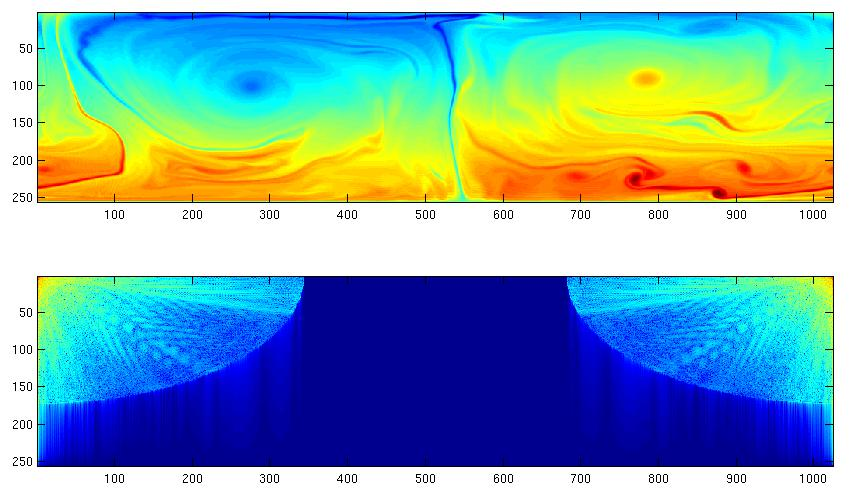
\includegraphics[width=0.9\textwidth, clip=true]{fouriervort}
    \end{center}
    \caption{Top: Vorticity field. Bottom: Spectral representation
    ($ln(1+abs(\xi))$). Note that some frequencies are just the complex
    conjugate of others.}
    \label{f:fouriervort}
    \end{figure}

This means that the vorticity can be expressed as:
    \PC{$a(l)_{k}$ stands for $a(y,t)_{k}$, \ie, coefficients carry spanwise
        and time dependence? Or what is this $l$?}
    \beq
    \xi(x,y)=\sum a(l)_{k} e^{-2 i \pi k x/M}
    \ee{120429_1}
So as stated in \refref{ACHKW11}, $\LieEl(\gSpace)=diag(e^{-2 \pi i k \gSpace /M})$
and $\Lg=diag(-2 \pi i k/M)$.

Now, the slice condition is given by $\LieEl( a_{kl}^T \gSpace(t))^T \Lg \slicep_{kl}$,
so I express the matrix as a vector:
    \beq
    a_{kl}=
    \begin{pmatrix}
    a_{11} & a_{12}& \cdots & a_{1N}&\cdots&a_{MN}\\
    \end{pmatrix}^T
    \ee{120429_2}
and carry out the slice condition, which looks something as:
    \bea
    \begin{pmatrix}
    a_{11} \\ a_{12}\\ \cdots \\ a_{1N}\\\cdots\\a_{MN}\\
    \end{pmatrix}^T
    \begin{pmatrix}
    e^{-2 \pi i \gSpace /M} & 0& \cdots & 0\\
    0 &  e^{-4 \pi i \gSpace /M}& \cdots & 0\\
    \vdots & \ddots& \ddots & \vdots\\
    0 & 0& \cdots & e^{-2 N \pi i \gSpace /M}
    \end{pmatrix}\\
    \continue
    \cdot
    \begin{pmatrix}
    -2 \pi i /M & 0& \cdots & 0\\
    0 &  -4 \pi i \gSpace /M& \cdots & 0\\
    \vdots & \ddots& \ddots & \vdots\\
    0 & 0& \cdots & -2 N \pi i  /M
    \end{pmatrix}
    \begin{pmatrix}
    \slicep_{11} \\ \slicep_{12}\\ \cdots \\ \slicep_{1N}\\\cdots\\\slicep_{MN}\\
    \end{pmatrix}^T = 0
    \label{120429_3}
    \eea
which after carrying it out gives me something as (but I have to check the algebra):
    \beq
    \LieEl(\gSpace(t))^T a_{kl}^T T \slicep_{kl}
     =\sum_{n=1} \left[n e^{-i n \gSpace}\left(\sum_{m=1}a_{mn}\slicep_{mn}\right)\right]=0
    \ee{120429_4}
I guess the next step would be to apply a Newton-Raphson to
\refeq{120429_4}. However, I am not sure how this would work, as the
equation have quite a large amount of terms, and has also an imaginary
component. Let me know if you have any advice for this.

Note: I will check the algebra tomorrow again; most likely I made an
embarrassing amount of mistakes while writing this. It is to late now.

\item[2012-04-29 Predrag]
You rotate only the fast Fourier transform for X, there is no
translational symmetry in the Y direction.

A vector is a vector, both in space and in Fourier space, so I do not see
why $a_{mn}$ became a matrix. Hope this helps (real form - complex is even
simpler):

Consider the general action of an
$\SOn{2}$ symmetry on arbitrary Fourier coefficients of a spatially
periodic function. Substituting this into the slice
condition
and using $g^{(m)}(\gSpace)=\cos(m\gSpace)\id^{(m)} +\sin(m\gSpace)
\frac{1}{m}\Lg^{(m)}$, we find that
\bea
\braket{e^{-\gSpace \Lg}\ssp}{\groupTan(\slicep)}
=\braket{\ssp}{\sum\limits_m \left(\cos(m\gSpace) \id^{(m)}
     +\sin(m\gSpace) \frac{1}{m}\Lg^{(m)}\right) \sliceTan{}}
\continue
=\sum\limits_m
   \left(
    \braket{\ssp}{\Lg^{(m)} \slicep} \cos(m\gSpace)
  - m\braket{\ssp}{\id^{(m)} \slicep} \sin(m\gSpace)
   \right)
   =0
\,.
\label{eq:so2sing}
\eea
This is a polynomial equation, with coefficients determined by
$\braket{\ssp}{\Lg^{(m)} \slicep}$ and $\braket{\ssp}{\id^{(m)}\slicep}$,
as we can see by rewriting $\cos(m\gSpace)$, $\sin(m\gSpace)$ as
polynomials of degree $m$ in $\sin(\gSpace)$ and $\cos(\gSpace)$. Each
phase $\gSpace$ that rotates $\ssp$ into any of the group-orbit
traversals of the slice hyperplane corresponds to a real root of this
polynomial.

It is fast - just a dot product, and as $\gSpace$ dependence is only in
the group element, the $d/d\gSpace$ derivative you need for Newton.
Complex Newton formula is the same as for real functions, thanks to
analyticity (analyticity assures that complex derivatives make sense).

\item[2012-04-30 Sebastian]
I do not understand why the transpose gets replaced by a complex
conjugate. I see in matlab what you mean by the transpose of the matrix.
But why does the complex conjugate gets involved in the transpose.

\item[2012-04-30 Predrag] If you are going to work in complex
representation, the norm of a complex vector $\ssp \in \complex^d$ is
$\norm{\ssp}^2 = \ssp^* \cdot \ssp$, and $(\LieEl\ssp)^*
=\ssp^*\LieEl^\dagger$, where $\LieEl^\dagger$ is the hermitian conjugate
= transpose + complex conjugate.

\item[2012-04-30 Predrag] Before getting into the Newton for this - make
sure that your $\LieEl(\gSpace)$ applied to a baroclinic state $\ssp$
does shift it by $\gSpace$, \ie,  $\LieEl(\gSpace)\ssp$ is the same $2D$
picture, but shifted by $\gSpace$.

\item[2012-04-30 Sebastian]
I have made a Matlab code that shifts the image by a $\gSpace$. Using
$\LieEl(\gSpace)=diag(e^{-2 \pi i k \gSpace /M})$. Looks as expected when converted
back to physical space.

\item[2012-04-30 Sebastian]
I reshape a matrix into a vector as Matlab's FFT works by columns. What I
have is a matrix that represents a vorticity field \SOA{which actually is
given as a vector from Annalisa's code, but I reshape it into a matrix
before doing anything in matlab} so what I do is to make a Fast Sine
Transform (FST) in Y and a FFT in X. This is something similar to
performing a 2D FFT. But to move all the fourier coefficients in X, I
reshape everything again as a vector. And then carry out the slicing
condition (all this in paper, in Matlab I have go up to the FFT transform
representation). So I think this would be equivalent only to a shift in
X.

Vector turns out to be huge, $262144$ dimensions for complex numbers; so
really is like $524288$ dimension. But a bit less than half of them are
just complex conjugates.

The term $a(l)_{k}$ means actually $a(l, t)_{k}$. I use it just to
emphasize that the transform in $x$, which is related with $k$, is
performed after a FST is made on the data for the $y$ direction. The
subindex $l$ is related to $y$. So $a(l)_{k}$, or perhaps better to write
$a_{lk}$, is a matrix (as shown in \reffig{f:fouriervort}), that I have
to reshape to rotate into the slice.  But I am not really sure why you
think it should be a vector.

\item[2012-04-30 Predrag]
Not sure why things got so huge? No point using Matlab for this - it is
fast and simple writing a dot product in C++ or Fortran. This is
Annalisa's department.

\item[2012-04-30 Sebastian]
I think the general procedure of what I did yesterday is OK. I have been
making the calculations this morning again. I believe is similar to what
you did in \refeq{eq:so2sing}, just that in complex space. By the way,
how do you get $e^{-\gSpace \Lg}$ to multiply $t'$ directly? Is it
because there should be a transpose in $e^{-\gSpace \Lg} x$?

\item[2012-04-30 Sebastian]
Advise greatly appreciated.

\item[2012-04-30 Predrag]
`advise' $\to$ `advice'.

\item[2012-04-30 Predrag] To view just the project (without this blog)
toggle the \texttt{boyscoutfalse} switch, towards the top of
\texttt{siminos/baroclinic/BrCv12.tex} file.

\item[2012-04-30 Sebastian]
How do you show that $\slicep^\dagger \Lg \slicep =0$?

\item[2012-04-30 Sebastian, Predrag]                                            \toCB
Unitary transformations preserve the magnitude of a complex vector
$\norm{\ssp} = \norm{\LieEl(\gSpace)\ssp}$, so $\LieEl^\dagger\LieEl=1$.
Expanding the norm to leading order in $\gSpace$
$\braket{(1+\gSpace\Lg)}{(1+\gSpace\Lg)}$ shows that the generators
are antihermitian, $\Lg^\dagger = - \Lg$, and from that it follows by complex conjugation
of the dot product $\ssp^\dagger \Lg \ssp$ that
$\ssp^\dagger \Lg \ssp =0$ for any vector $\ssp \in \reals^d$.

To evaluate the slice condition for unitary groups,
\beq
\frac{\partial}{\partial \gSpace} \norm{\ssp-\LieEl\slicep}^2 =0
\,,
\ee{120429_5}
start by expanding
\[
    (\ssp-\LieEl\slicep)^\dagger (\ssp-\LieEl\slicep)
= \norm{\ssp}^2
  - \slicep^\dagger\LieEl^\dagger\ssp - \ssp^\dagger\LieEl\slicep
  + \norm{\slicep}^2
\]
 so
\bea
\frac{\partial}{\partial \gSpace}
    (\ssp-\LieEl\slicep)^\dagger (\ssp-\LieEl\slicep)
&=& -\frac{\partial}{\partial \gSpace}
(\slicep^\dagger\LieEl^\dagger\ssp + \ssp^\dagger\LieEl\slicep)
 = -2\,\Re \left(\ssp^\dagger \frac{\partial \LieEl}{\partial \gSpace} \slicep\right)
\continue
&=& - 2\,\Re \left(\ssp^\dagger \LieEl \Lg \slicep\right)
\,.
\label{120429_6}
\eea
Substitute $\ssp=\LieEl\sspRed$.
    \PC{This is OK for abelain groups, as along the way I assumed $\LieEl
    \Lg = \Lg\LieEl $, but have to redo it more carefully for nonabelian
    groups.}
This yields the \emph{slice condition} for unitary groups:
\beq
    \Re(\sspRed^\dagger \Lg \slicep)=0
\ee{120430_11}

%\beq
%\frac{\partial}{\partial \gSpace}
%\left(\ssp^\dagger a - a^\dagger g\slicep -(g\slicep )^\dagger a+(g\slicep)^\dagger g\slicep \right)
%\,,
%\ee{120429_7}
%carrying out the derivative, nothing that $\partial g/\partial \gSpace =
%\Lg g$ and grouping terms I arrive to:
%\beq
%(\ssp-g\slicep)^\dagger \Lg \LieEl\slicep +(\Lg \LieEl\slicep)^\dagger (\ssp-g\slicep )=0
%\,.
%\ee{120429_8}
%As both terms are a complex numbers and one is the complex conjugate of
%the other, this means that the imaginary term vanish and the condition
%can be written:
%\beq
%2 \Re[(\ssp-g\slicep)^\dagger \Lg \LieEl\slicep ]=0
%\,,
%\ee{120429_9}
%and $a=g\widehat{\ssp}$, so that
%\beq
%2 \Re[(\widehat{\ssp}-\slicep)^\dagger g^\dagger \Lg \LieEl\slicep]=0
%\ee{120429_10}
%but
%$g^\dagger=diag[\overline{e^{-im\gSpace}}]=diag[e^{\overline{-im\gSpace}}]
%=diag[e^{im\gSpace}]$ so that $g^\dagger \Lg g=\Lg$ an the condition becomes:
%\beq
%2 \Re[(\widehat{\ssp}-\slicep)^\dagger \Lg \slicep ]=0
%\ee{120429_11}

One use this condition for Newton-Raphson determination of \sspRed.

\item[2012-04-30 Sebastian]
I tried to run the model changing the resolution, but results
do not look \PCedit{good}. Not much happened, energy did not traveled up scale.
Small scales are important. I think the simulation starts looking good
from $512 \times 128$ so I might change to that one. But there is always the
chance that I did not change some parameter in the simulation needed when
changing scales. I would have to check with Annalisa.

\item[2012-04-30 Sebastian]
Not sure $\ssp^\dagger \Lg \ssp$ vanishes, although it is antihermitian
it is a diagonal matrix. I think the correct answer is:
\beq
\ssp^\dagger \Lg \ssp = - \sum_{l=1} \sum_{k=1} i k \| \ssp_{l,k}\|^2
\ee{anti-antihermiticity}
Let me know if I am missing something.

\item[2012-05-01 Predrag]
Maybe elementary, student Ortega. Take $[1\!\times\!1]$ antihermitian matrix $\Lg = \ii$.
It's diagonal, right. And  $\Lg^\dagger = - \ii$. If we did this as $\SOn{2}$ there would be
no confusion, but with $\Un{1}$ one tends to get confused. BTW, there is no sum on $l$ in
\refeq{anti-antihermiticity} - it vanishes for every value of $l$ separately.

$\ssp^\dagger \Lg \ssp= (x-\ii y)\ii (x+\ii y) = $

\item[2012-04-30 Sebastian]
Ok. So a'+Ta' vanishes? I do not see it. I can go by your office and tell
you how I derive it, maybe you can tell me where I went wrong. The sum in
l is an artifact of how I derived things.

\item[2012-05-1 Sebastian]
Finish writing a very quick draft of the non linear section.

\item[2012-05-1 Sebastian]
Did some tweaking for the final project. Now it is in final form. I did
not have time to check all equations, but I guess they are ok. I will go
after Thursday trough the derivation of \refeq{min4} and run the
algorithm to see what happens.

I think it turn out ok. I like the final result. Let me know what you
think. As usual comments are greatly appreciated.

\item[2012-05-4 Sebastian]
I have been trying to implement the slicing condition of the term
project. Newton method converges and it is quite fast, even for the
1024x256 runs. However, it always converges very near the initial guess,
so that something is wrong. I was also thinking of how is one to
implement the border condition given that we are dealing with complex
numbers.

\item[2012-04-30 Predrag] If you are going small steps in time, this
sound correct - the in-slice trajectory will be close to the full space
trajectory. You just have to be sure that all points on it satisfy the
slice condition.

\item[2012-05-04 Sebastian] Let me know if you have any advise for any of
these points.

\item[2012-04-30 Predrag]
`advise' $\to$ `advice'.


\item[2012-05-04 Sebastian]
I spotted some things I can correct in my final work (minor changes), let
me know if changes are still allowed.

\item[2012-04-30 Predrag]
Keep editing and improving it - I can always post improved version on
\HREF{http://ChaosBook.org/projects}{ChaosBook.org/projects}. As far as I
am concerned, this project is not over until either the fat lady sings,
or you slice the baroclinic instability.


\end{description}
